The course notes develop the point-force modal expansion and frequency-response function (FRF) on PDF pages 164--170. With $U_j(x)=\sin(j\pi x/L)$, each modal mass is $m_j=mL/2$. The mode shapes below are normalized to unit peak displacement.

\textbf{A.6.1--A.6.3. Input and modal properties.} The inputs are $L=25.5\,\mathrm{in}=0.6477\,\mathrm{m}$, $m=0.00150\,\mathrm{kg/m}$, $\zeta_j=0.021$, $F_e=0.500\,\mathrm{N}$, $N=10$, and 5000 frequency samples from 20 to 2000 Hz. The note G3 has $f_1=196.0\,\mathrm{Hz}$, so
\[
\tau_1=\frac1{f_1}=5.102\,\mathrm{ms},\quad
c=2Lf_1=253.9\,\mathrm{m/s},\quad
m_j=\frac{mL}{2}=0.4858\,\mathrm{g}.
\]
The modal wavenumbers and angular frequencies follow from $\gamma_j=j\pi/L$ and $\omega_j=2\pi jf_1$. The modal mass results from integrating the distributed mass against the squared unit-peak mode shape,
\[
m_j=\int_0^L m\sin^2\!\left(\frac{j\pi x}{L}\right)dx
=\frac{mL}{2}=4.85775\times10^{-4}\ \mathrm{kg}.
\]
The table gives the ten modal properties. Every damping ratio is $\zeta_j=0.021$ and every modal mass is $m_j=0.4858\ \mathrm{g}$.
\begin{center}\small
\begin{tabular}{rrrr}
\toprule
$j$ & $\gamma_j$ (rad/m) & $\omega_j$ (rad/s) & $f_j$ (Hz)\\
\midrule
1 & 4.850 & 1231.5 & 196\\
2 & 9.701 & 2463.0 & 392\\
3 & 14.551 & 3694.5 & 588\\
4 & 19.402 & 4926.0 & 784\\
5 & 24.252 & 6157.5 & 980\\
6 & 29.102 & 7389.0 & 1176\\
7 & 33.953 & 8620.5 & 1372\\
8 & 38.803 & 9852.0 & 1568\\
9 & 43.653 & 11083.5 & 1764\\
10 & 48.504 & 12315.0 & 1960\\
\bottomrule
\end{tabular}
\end{center}

\begin{figure}[H]\centering
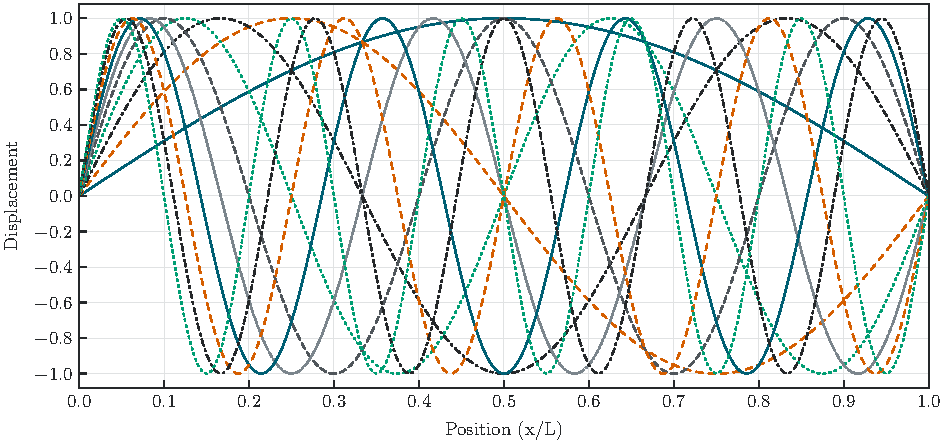
\includegraphics[width=0.80\linewidth]{figures/generated/solutions/A6-modes.pdf}
\caption{A.6.3. First ten string mode shapes.}
\end{figure}

\textbf{A.6.4--A.6.5. Frequency response.} The frequency grid is $f=\operatorname{linspace}(20,2000,5000)$ Hz and $\omega=2\pi f$. A point force $F_e e^{i\omega t}$ at $x_e$ contributes the generalized force $F_eU_j(x_e)$ to mode $j$. The equation for its modal coordinate is
\[
m_j\ddot q_j+2\zeta_j\omega_jm_j\dot q_j
 +m_j\omega_j^2q_j=F_eU_j(x_e)e^{i\omega t}.
\]
For steady harmonic motion, set $q_j=Q_je^{i\omega t}$. The resulting modal amplitude is
\[
Q_j=\frac{F_eU_j(x_e)}
{m_j(\omega_j^2-\omega^2+2i\zeta_j\omega_j\omega)}.
\]
Summing $Q_jU_j(x_0)$ at the pickup and dividing by $F_e$ gives the displacement receptance using the notes' $e^{i\omega t}$ convention,
\[
H(\omega;x_e,x_0)=\sum_{j=1}^{10}
\frac{U_j(x_0)U_j(x_e)}
{m_j(\omega_j^2-\omega^2+2i\zeta_j\omega_j\omega)}.
\]
The plotted quantity is $20\log_{10}(|H|/(1\,\mathrm{m/N}))$. The applied force gives displacement amplitude $F_e|H|$.

\begin{figure}[H]\centering
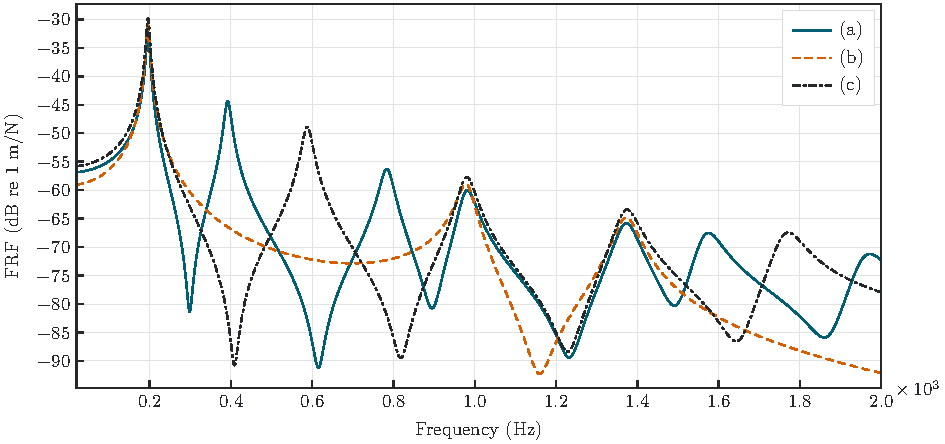
\includegraphics[width=0.80\linewidth]{figures/generated/solutions/A6-frf.pdf}
\caption{A.6.5. Displacement FRF for the three excitation and pickup locations.}
\end{figure}

The sampled local peaks with at least 1 dB prominence, nearest equal-tempered notes, and mode indices are listed below. Peak frequencies shift slightly from modal frequencies because neighboring modes contribute.

\begin{center}\small
\begin{tabular}{@{}clll@{}}\toprule
Case & Peak frequencies (Hz) & Nearest notes & Mode indices \\ \midrule
(a) & 195.9, 391.9, 783.2, 982.1 & G3, G4, G5, B5 & 1, 2, 4, 5 \\
    & 1373, 1575, 1972 & F6, G6, B6 & 7, 8, 10 \\
(b) & 195.9, 977.7, 1373 & G3, B5, F6 & 1, 5, 7 \\
(c) & 195.9, 588.0, 980.5, 1375, 1771 & G3, D5, B5, F6, A6 & 1, 3, 5, 7, 9 \\
\bottomrule\end{tabular}\end{center}
The numerator determines which modes can be excited and measured. At $L/3$, $U_j(L/3)=\sin(j\pi/3)$ vanishes for multiples of three. At the midpoint, $U_j(L/2)=\sin(j\pi/2)$ vanishes for even modes. Consequently case (b) excludes both sets, and case (c) retains only odd modes. Damping and the combined modal response affect the locations of the observed peaks.

\textbf{A.6.6. Pickup response.} Case (b) is strongest at $f_d=195.9\,\mathrm{Hz}$ on the specified grid. The steady harmonic displacement is $u(t)=\Re\{F_eH(2\pi f_d)e^{i2\pi f_dt}\}$. At this sampled frequency, the sum gives
\[
H(2\pi f_d)=0.0008841-0.027975i\ \mathrm{m/N},\qquad
|H|=0.027989\ \mathrm{m/N},\qquad \arg H=-1.5392\ \mathrm{rad}.
\]
The corresponding pickup amplitude is $F_e|H|=0.01399\ \mathrm{m}$. Dividing by this amplitude gives
\[
\frac{u(t)}{F_e|H|}=\cos(2\pi f_dt-1.5392),
\qquad 0\leq t\leq\frac{3}{f_d}=15.32\ \mathrm{ms}.
\]
This expression retains the phase of the pickup motion relative to the applied force.

\begin{figure}[H]\centering
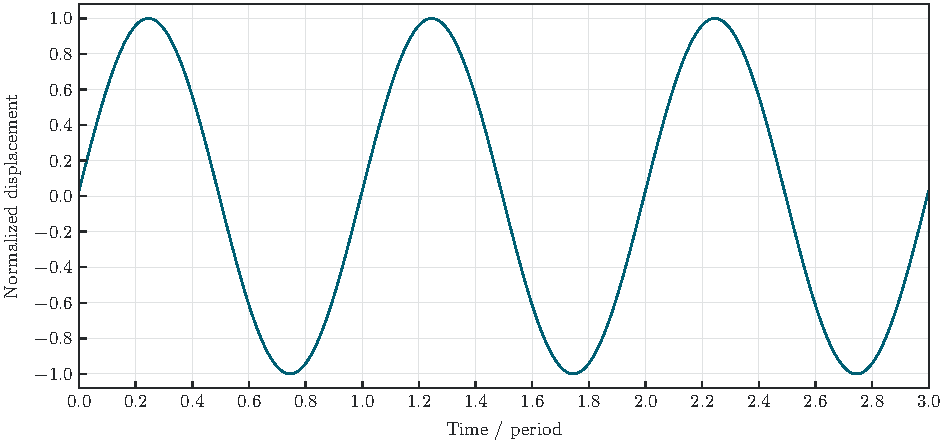
\includegraphics[width=0.80\linewidth]{figures/generated/solutions/A6-time.pdf}
\caption{A.6.6. Normalized pickup displacement for case (b) at the dominant frequency.}
\end{figure}
\lstinputlisting[style=hwmatlab,caption={A.6. MATLAB modal expansion and frequency-response calculation.}]{matlab/A6.m}
